\documentclass[]{book}

\usepackage{import}
\usepackage{preamble}
\usepackage{tikz}

\begin{document}

\noindent BECA / Huson / 11.1 IB Math SL \hspace{2in} Name:\\*
16 November 2017
\begin{center}
{\Large Quiz: Exponents and radicals}\\
\textit{Work without a calculator. Answer in the space provided.}
\end{center}

%\vspace{0.2 cm}


Simplify, leaving no negative or fractional exponents.

\begin{enumerate}

\item $7a^{-5}b^2 \times 2a^3 b^{-2}$\\*[65pt]
\item $\sqrt[3]{8x^9 y}$\\*[65pt]
\item $\displaystyle a^{\frac{2}{3}} \times (\frac{16 a^{-2}}{b^4})^{\frac{1}{2}}$\\*[75pt]
\item $\displaystyle (x^6 y^4)^{\frac{1}{3}} \div x^{-2} y$\\*[55pt]

\newpage
\item State whether this relation is a function. Justify your answer. $\{(3, 4),(5,6), (3, -4), (6, -6)\}$\\*[45pt]
\item Graph the function $f(x) = (x+1)^2 - 4$ over the domain $x \geq -1$ on the grid below. 
\begin{enumerate}
    \item Label the $y$-intercept as an ordered pair.
    \item Label the point representing the solution to the equation $f(x)=0$ as an ordered pair.\\*[25pt]
    \item Find the inverse function of $f(x)$.\\*[25pt]
    \item Graph the inverse function, $f^{-1}(x)$.\\*[15pt]
\end{enumerate}

\begin{figure}[!htbp]
\begin{center}
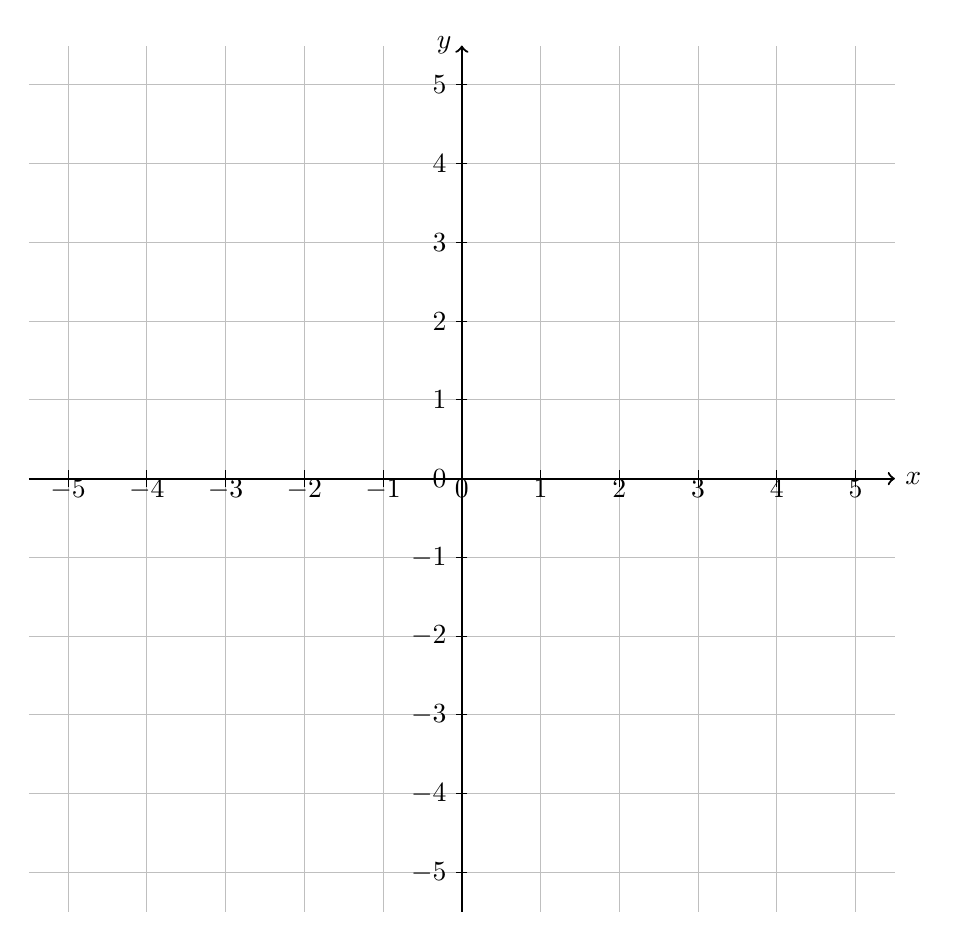
\begin{tikzpicture}

%grid
\draw [thin, color=lightgray,, xstep=1.0cm,ystep=1.0cm] (-5.5,-5.5) grid (5.5,5.5);
%\draw [thin, color=lightgray,, xstep=0.2cm,ystep=0.2cm] (-5.5,-1.5) grid (5.5,16.5);

\foreach \x in {-5, -4, -3, -2, -1, 0,1,2,3,4,5}
\draw[shift={(\x,0)},color=black] (0pt,-3pt) -- (0pt,3pt) node[below]  {$\x$};

\foreach \y in {-5, -4, -3, -2, -1, 0,1,2,3,4,5}
\draw[shift={(0,\y)},color=black] (2pt,0pt) -- (-2pt,0pt) node[left]  {$\y$};

\draw [thick, ->] (-5.5,0) -- (+5.5,0) node [right] {$x$};
\draw [thick, ->] (0,-5.5) -- (0,5.5) node [left] {$y$};

%\draw plot[domain= -1:3] (\x, (\x+1)*(\x+1) - 4);

\end{tikzpicture}
\end{center}
\end{figure}


\end{enumerate}

\end{document}